\section{Évaluation de l'hypothèse de robustesse}
\label{section:4.6-HYPOTHESE-ROBUSTESSE}

	%%% Introduction / Transition.
	Dans les précédentes études, nous avons presque toujours analysé le \textit{clustering} interactif en supposant que l'annotateur connaît parfaitement le domaine traité par le jeu de données et qu'il est capable de caractériser sans ambiguïté la similitude entre deux données issues de cet ensemble.
	Bien entendu, cette hypothèse forte n'est pas toujours vérifiée en situation réelle : l'interprétation du langage peut contenir certaines ambiguïtés, l'opérateur peut faire des erreurs d’inattention, et deux annotateurs peuvent avoir des avis contraire sur un même sujet.
	Or, comme notre méthode d'annotation est itérative, elle est a priori sensible aux dérives fonctionnement liées à ce type de contradictions.
	Dans cette section, nous nous intéresserons donc à la robustesse du \textit{clustering} interactif en présence d'incohérences dans les contraintes et aux moyens de les contrer.
	Pour cela, nous aimerions donc vérifier l'hypothèse suivante :
	
	%%% Formulation des hypothèses:
	\begin{tcolorbox}[
		title=\faVial~\textbf{Hypothèse de robustesse}~\faVial,
		colback=colorTcolorboxHypothesis!15,
		colframe=colorTcolorboxHypothesis!75,
		width=\linewidth
	]
		% Hypothèse.
		\textguillemets{\textbf{
			Au cours d'une méthodologie d'annotation basée sur le \textit{clustering} interactif, il est possible d'estimer le taux d'incohérences dans les contraintes ainsi que leur impact sur les performances de la méthode.
		}} \\
		
		% Figure.
		La \textsc{Figure~\ref{figure:4.6-HYPOTHESE-ROBUSTESSE}} illustre cette hypothèse et l'espoir de estimer l'impact différences ou d'erreurs d'annotations sur le nombre d'itérations de la méthode.
		%
		\begin{figure}[H]  % keep [H] to be in the tcolorbox.
			\centering
			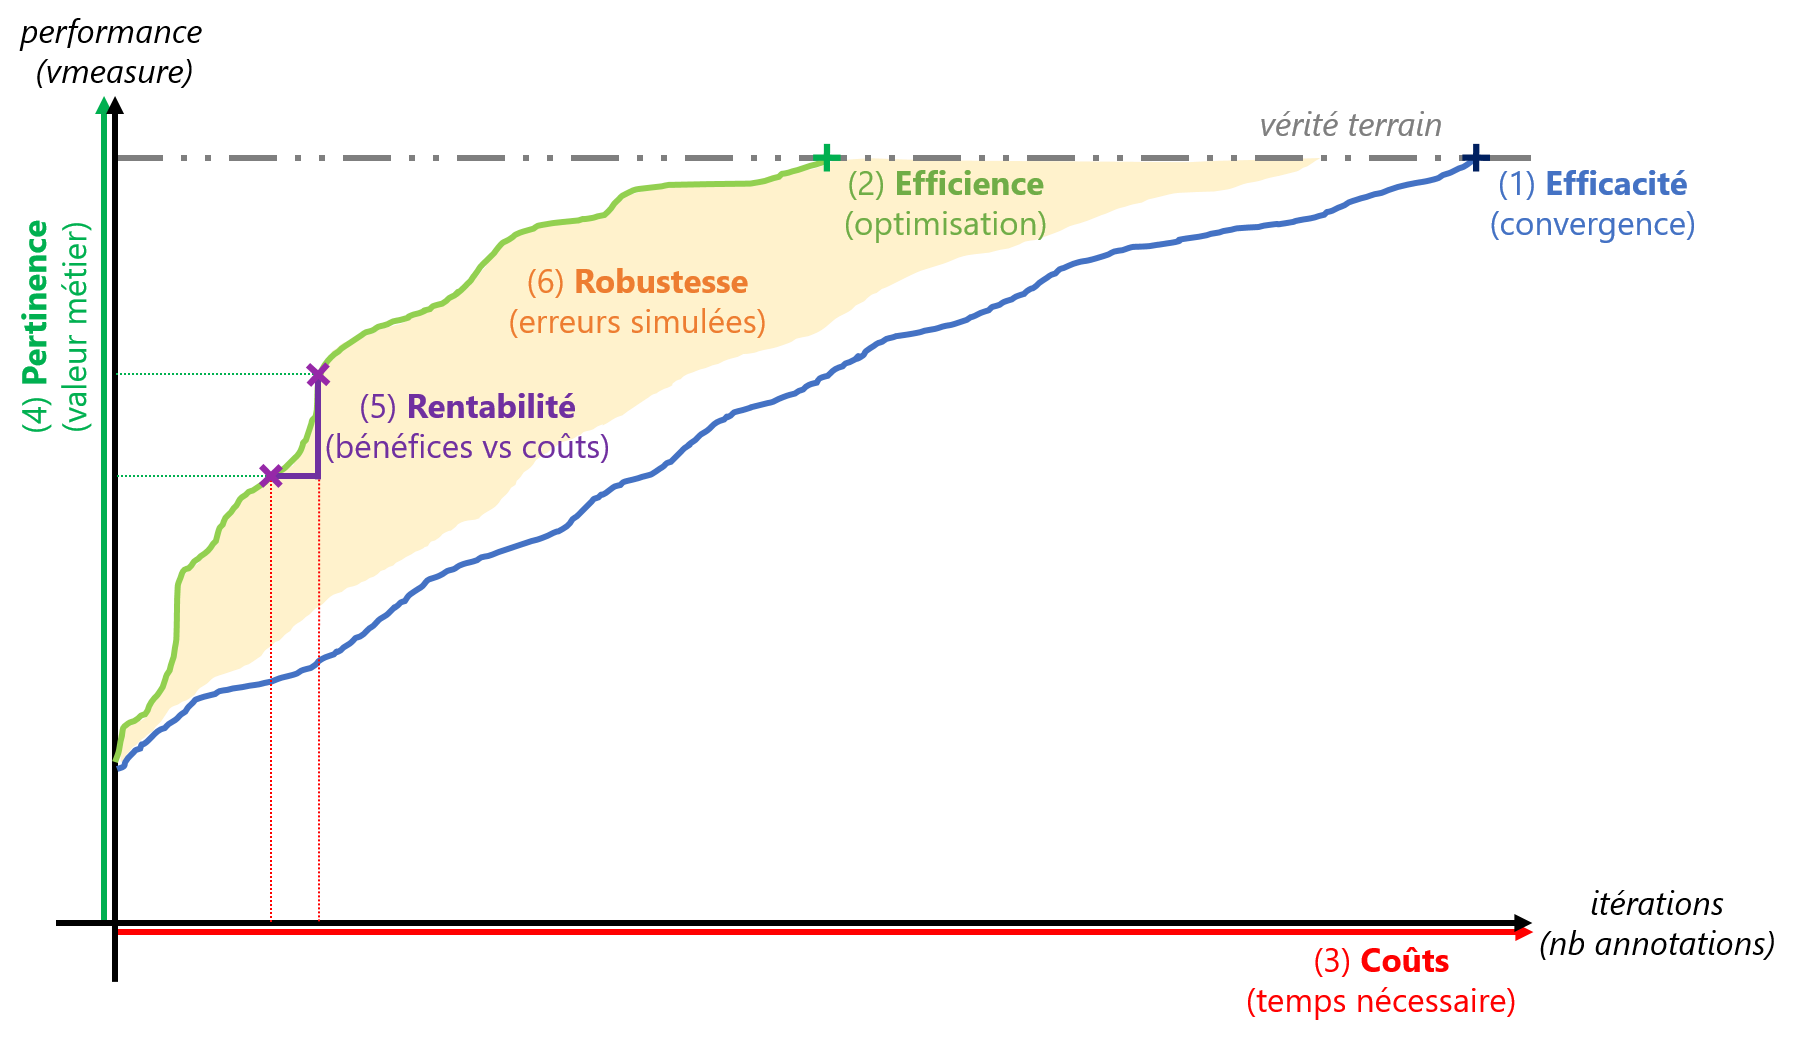
\includegraphics[width=0.95\textwidth]{figures/hypotheses-06-robustesse}
			\caption{
				Illustration des études réalisées sur le \textit{clustering} interactif (\textit{étape 6/6}) en schématisant l'évolution de la pertinence (\textit{valeur métier évaluée par l'expert et exprimé en nombre de clusters}) d'une base d'apprentissage en cours de construction en fonction du coût temporel de la méthode (\textit{temps nécessaire à l'expert métier et à la machine}), ainsi que les marges d'erreurs représentant l'impact de différences d'annotation sur le nombre d'itérations nécessaire à la méthode.
			}
			\label{figure:4.6-HYPOTHESE-ROBUSTESSE}
		\end{figure}
	\end{tcolorbox}
		
	% Résumé de l'étude.
	Afin de vérifier cette hypothèse, nous organisons trois expériences :
	\begin{itemize}
		\item une étude de cas sur la \textbf{correction des incohérences d'annotation} (cf. \textsc{Section~\ref{section:4.6.1-ETUDE-ROBUSTESSE-INTERETS-CORRECTION-ERREURS}}) ;
		\item une simulation de l'\textbf{impact des incohérences d'annotation} sur les performances de la méthode (cf. \textsc{Section~\ref{section:4.6.2-ETUDE-ROBUSTESSE-SIMULATION-IMPACT-ERREURS}}) ;
		\item une étude de cas sur le \textbf{score inter-annotateurs} obtenu lors d'une annotation de contraintes en situation réelle avec plusieurs opérateurs (cf. \textsc{Section~\ref{section:4.6.3-ETUDE-ROBUSTESSE-SCORE-INTER-ANNOTATEURS}}).
	\end{itemize}
	
	
	%%%
	%%% Subsection 4.6.1: Étude de l'intérêt de la correction des incohérences d'annotation.
	%%%
	\subsection{Étude de l'intérêt de la correction des incohérences d'annotation}
	\label{section:4.6.1-ETUDE-ROBUSTESSE-INTERETS-CORRECTION-ERREURS}
		
		% Objectif de l'expérience.
		Nous cherchons à estimer la robustesse du \textit{clustering} interactif face aux incohérences d'annotation.
		Dans cette étude, nous nous intéressons plus particulièrement à l'intérêt de la détection et de la correction des conflits présents dans les contraintes.
		En effet, deux approches de travail s'opposent :
		\begin{itemize}
			\item une approche naïve ignorant simplement les conflits : celle-ci n'engendre pas de coûts supplémentaires, mais elle s'expose aux risques de dérives de fonctionnement ;
			\item une seconde approche avec correction des conflits : celle-ci nécessite de revoir ou de ré-annoter des contraintes, impliquant un coût supplémentaire, mais permet de limiter l'impact de dérives potentielles.
		\end{itemize}
		Pour trancher entre ces deux options, nous simulons ces deux approches afin d'estimer si l'absence de correction induit une régression significative des performances de notre méthode d'annotation.
	
		%%% Protocole expérimental.
		\subsubsection{Protocole expérimental}
			
			% Pseudo-code.
			Pour résumer le protocole expérimental que nous décrivons ci-dessous, vous pouvez vous référer au pseudo-code décrit dans \textsc{Algorithme~\ref{algorithm:4.6.1-ETUDE-ROBUSTESSE-INTERETS-CORRECTION-ERREURS-PROTOCOLE}}.
			\todo{FORMAT: ajuster l’enchaînement pour ne pas avoir de page "blanche" avec l'algorithme.}
			
			\begin{algorithm}
				\KwData{jeu de données annoté (vérité terrain)}
				\KwIn{taux d'erreurs à tester}
				%
				\ForEach{arrangement de taux d'erreur à tester}{
					\textbf{initialisation (données)}: récupérer les données et la vérité terrain \;
					\textbf{initialisation (contraintes)}: créer une liste vide de contraintes \;
					\textbf{prétraitement}: supprimer le bruit dans les données avec \texttt{prep.simple} \;
					\textbf{vectorisation}: transformer les données en vecteurs avec \texttt{vect.tfidf} \;
					\textbf{clustering initial}: regrouper les données par similarité avec \texttt{clust.kmeans.cop} \;
					\textbf{évaluation}: estimer l'équivalence entre le \textit{clustering} obtenu et la vérité terrain \;
					\Repeat{annotation de toutes les contraintes possibles}{
						\textbf{échantillonnage}: sélectionner des contraintes avec \texttt{samp.closest.diff} \;
						\textbf{échantillonnage d'erreurs}: définir les contraintes qui seront erronées \;
						\textbf{simulation d'annotation}: caractériser les contraintes grâce à la vérité terrain \;
						\If{absence de correction des conflits d'annotation}{
							\textbf{intégration naïve}: ignorer les conflits avec le gestionnaire de contraintes \;
						}
						\ElseIf{détection et correction des conflits d'annotation}{
							\textbf{intégration corrective}: changer les annotations erronées en conflit \;
						}
						\textbf{clustering}: regrouper les données par similarité avec \texttt{clust.kmeans.cop} \;
						\textbf{évaluation}: estimer l'équivalence entre le \textit{clustering} obtenu et la vérité terrain \;
					}
				}
				\textbf{analyse}: déterminer l'impact par itération et par taux d'erreurs de la correction \;
				%
				\KwResult{discussion sur l'impact de la correction des incohérences}
				%
				\caption{\textit{
					Description en pseudo-code du protocole expérimental de l'étude d'intérêt de la correction des incohérences d'annotation.
				}}
				\label{algorithm:4.6.1-ETUDE-ROBUSTESSE-INTERETS-CORRECTION-ERREURS-PROTOCOLE}
			\end{algorithm}
			
			% Description de la vérité terrain.
			Nous utilisons comme vérité terrain le jeu de données \texttt{Bank Cards (v1.0.0)} : ce dernier traite des demandes les plus fréquentes des clients en ce qui concerne la gestion de leur carte bancaire.
			Il est composé de $500$ questions rédigées en français et réparties en $10$ classes (\texttt{perte ou vol de carte}, \texttt{carte avalée}, \texttt{commande de carte}, ...).
			Pour plus de détails, consultez l'annexe~\ref{annex:C.1-DATASET-BANK-CARDS}.
			
			% Description des tentatives de la méthode avec simulation d'erreurs.
			Sur ce jeu de données, nous exécutons une tentative complète
			\footnote{Tentative complète : itérations d'échantillonnage, d'annotation et de \textit{clustering} jusqu'à annotation de toutes les contraintes possibles.}
			de la méthode du \textit{clustering} interactif en utilisant notre paramétrage favori (voir \textsc{Section~\ref{section:4.4.3-ETUDE-PERTINENCE-RESUME-AUTOMATIQUE}}).
			Toutefois, contrairement aux précédents expériences, nous allons ajouter un pourcentage de contraintes erronées à chaque itération :
			\begin{itemize}
				\item Le taux d'erreurs insérées, variant de $0$\% à $50$\% par pas de $5$\%, reste fixe tout au long d'une même tentative de notre méthode : nous pouvons ainsi analyser l'impact d'un taux d'erreur fixe sur les performances au courant des itérations ;
				\item Les contraintes erronées à insérer sont tirées aléatoirement parmi le lot de contraintes qui aurait été échantillonné au cours d'une tentative sans erreur : ainsi, nous pouvons comparer itération par itération toutes ces simulations car elles partagent la même base de contraintes (aux valeurs de \texttt{MUST-LINK} et \texttt{CANNOT-LINK} près) ;
			\end{itemize}
			
			% Description des tentatives de la méthode avec gestion des conflits.
			Puisque nous introduisons des erreurs d'annotations, des conflits vont apparaître dans le gestionnaire de contraintes.
			Pour rappel, un conflit est détecté dans le cas où l'ajout d'une nouvelle contrainte annotée contredit ce qui a été précédemment déduit grâce aux propriétés de transitivité des contraintes de types \texttt{MUST-LINK}et \texttt{CANNOT-LINK} (voir \textsc{Figure~\ref{figure:3.3-CONTRAINTES-TRANSITIVITE}} en \textsc{Section~\ref{section:3.3.2-GESTION-DES-CONTRAINTES}}).
			Pour les traiter, nous testons deux approches :
			\begin{itemize}
				\item l'approche naïve ignorant simplement les conflits : si la prochaine contrainte à ajouter est incompatible avec la base de contraintes déjà intégrées au gestionnaire, alors nous ignorons simplement son existence sans remettre en question les précédentes annotations ;
				\item l'approche avec correction des conflits : pour simuler la correction d'un expert, nous recréons à chaque itération le gestionnaire de contraintes en intégrant d'abord les contraintes correctes puis les contraintes erronées ; ainsi, les conflits ne peuvent arrivent qu'à l'ajout d'une contrainte erronée, et il suffit d'ajouter sa version exacte pour simuler la correction de l'expert.
			\end{itemize}
			
			% Description des tentatives de la méthode avec les répétitions.
			Ainsi, il y a donc $11$ taux d'erreurs différents à simuler, chacun suivant $2$ approches de gestion de conflits différentes, et chacune de ces simulations d'erreurs seront répétées $10$ fois sur chaque tentative complète de la méthode pour limiter contrer les aléas statistiques des tirages de contraintes erronées, ce qui représente $220$ simulation par tentatives.
			Enfin, chaque tentative complète de \textit{clustering} interactif est répétée $5$ fois pour contrer les aléas statistiques des exécutions, ce qui représente un total de $1100$ tentatives complètes à simuler.

			% Description de l'analyse.
			Enfin, nous afficherons l'évolution de la performance moyenne du \textit{clustering} obtenu en fonction des divers taux d'erreurs simulés, et discuterons de l'impact au cours des itérations de la présence ou de l'absence de corrections des conflits d'annotations détectés.
			
			% Référence scripts.
			\begin{leftBarInformation}
				Les scripts de l'expérience, réalisés avec des \textit{notebooks} Python (\cite{van-rossum-drake:2009:python-reference-manual}), sont disponibles dans un dossier dédié de~\cite{schild:2021:cognitivefactory-interactiveclusteringcomparativestudy}.
			\end{leftBarInformation}

		%%% Résultats
		\subsubsection{Résultats obtenus}
		
			% Description statistiques.
			La \textsc{Figure~\ref{figure:4.6.1-ETUDE-ROBUSTESSE-INTERETS-CORRECTION-ERREURS}} représente l'évolution moyenne de la \texttt{v-measure} du \textit{clustering} en fonction du nombre d'itération de la méthode, déclinée avec les $11$ taux d'erreurs simulés et les $2$ approches de gestion des conflits.
			Les contraintes utilisées sont basées sur les échantillonnages réalisées au cours des tentatives sans erreurs : comme les mêmes contraintes sont donc utilisées (aux valeurs d'annotations près), toutes les courbes sont comparables point par point.
			
			\begin{leftBarWarning}
				Toutefois, il est important de noter que les tentatives sans contraintes ont besoin de maximum $3~000$ contraintes pour annoter toutes les contraintes possibles et leurs transitivités (moyenne: $2~488$, écart-type: $327$).
				Ainsi, toutes les courbes simulant les différents taux d'erreurs sont tronquées à $3~000$ contraintes, que les tentatives aient convergé ou non.
				Nous serons sensible à cette information pour ne pas faire de mauvaises interprétations, car le dernier point des différentes courbes ne représente pas forcément le point de convergence des tentatives associées.
			\end{leftBarWarning}
			
			\begin{figure}[!htb]
				\centering
				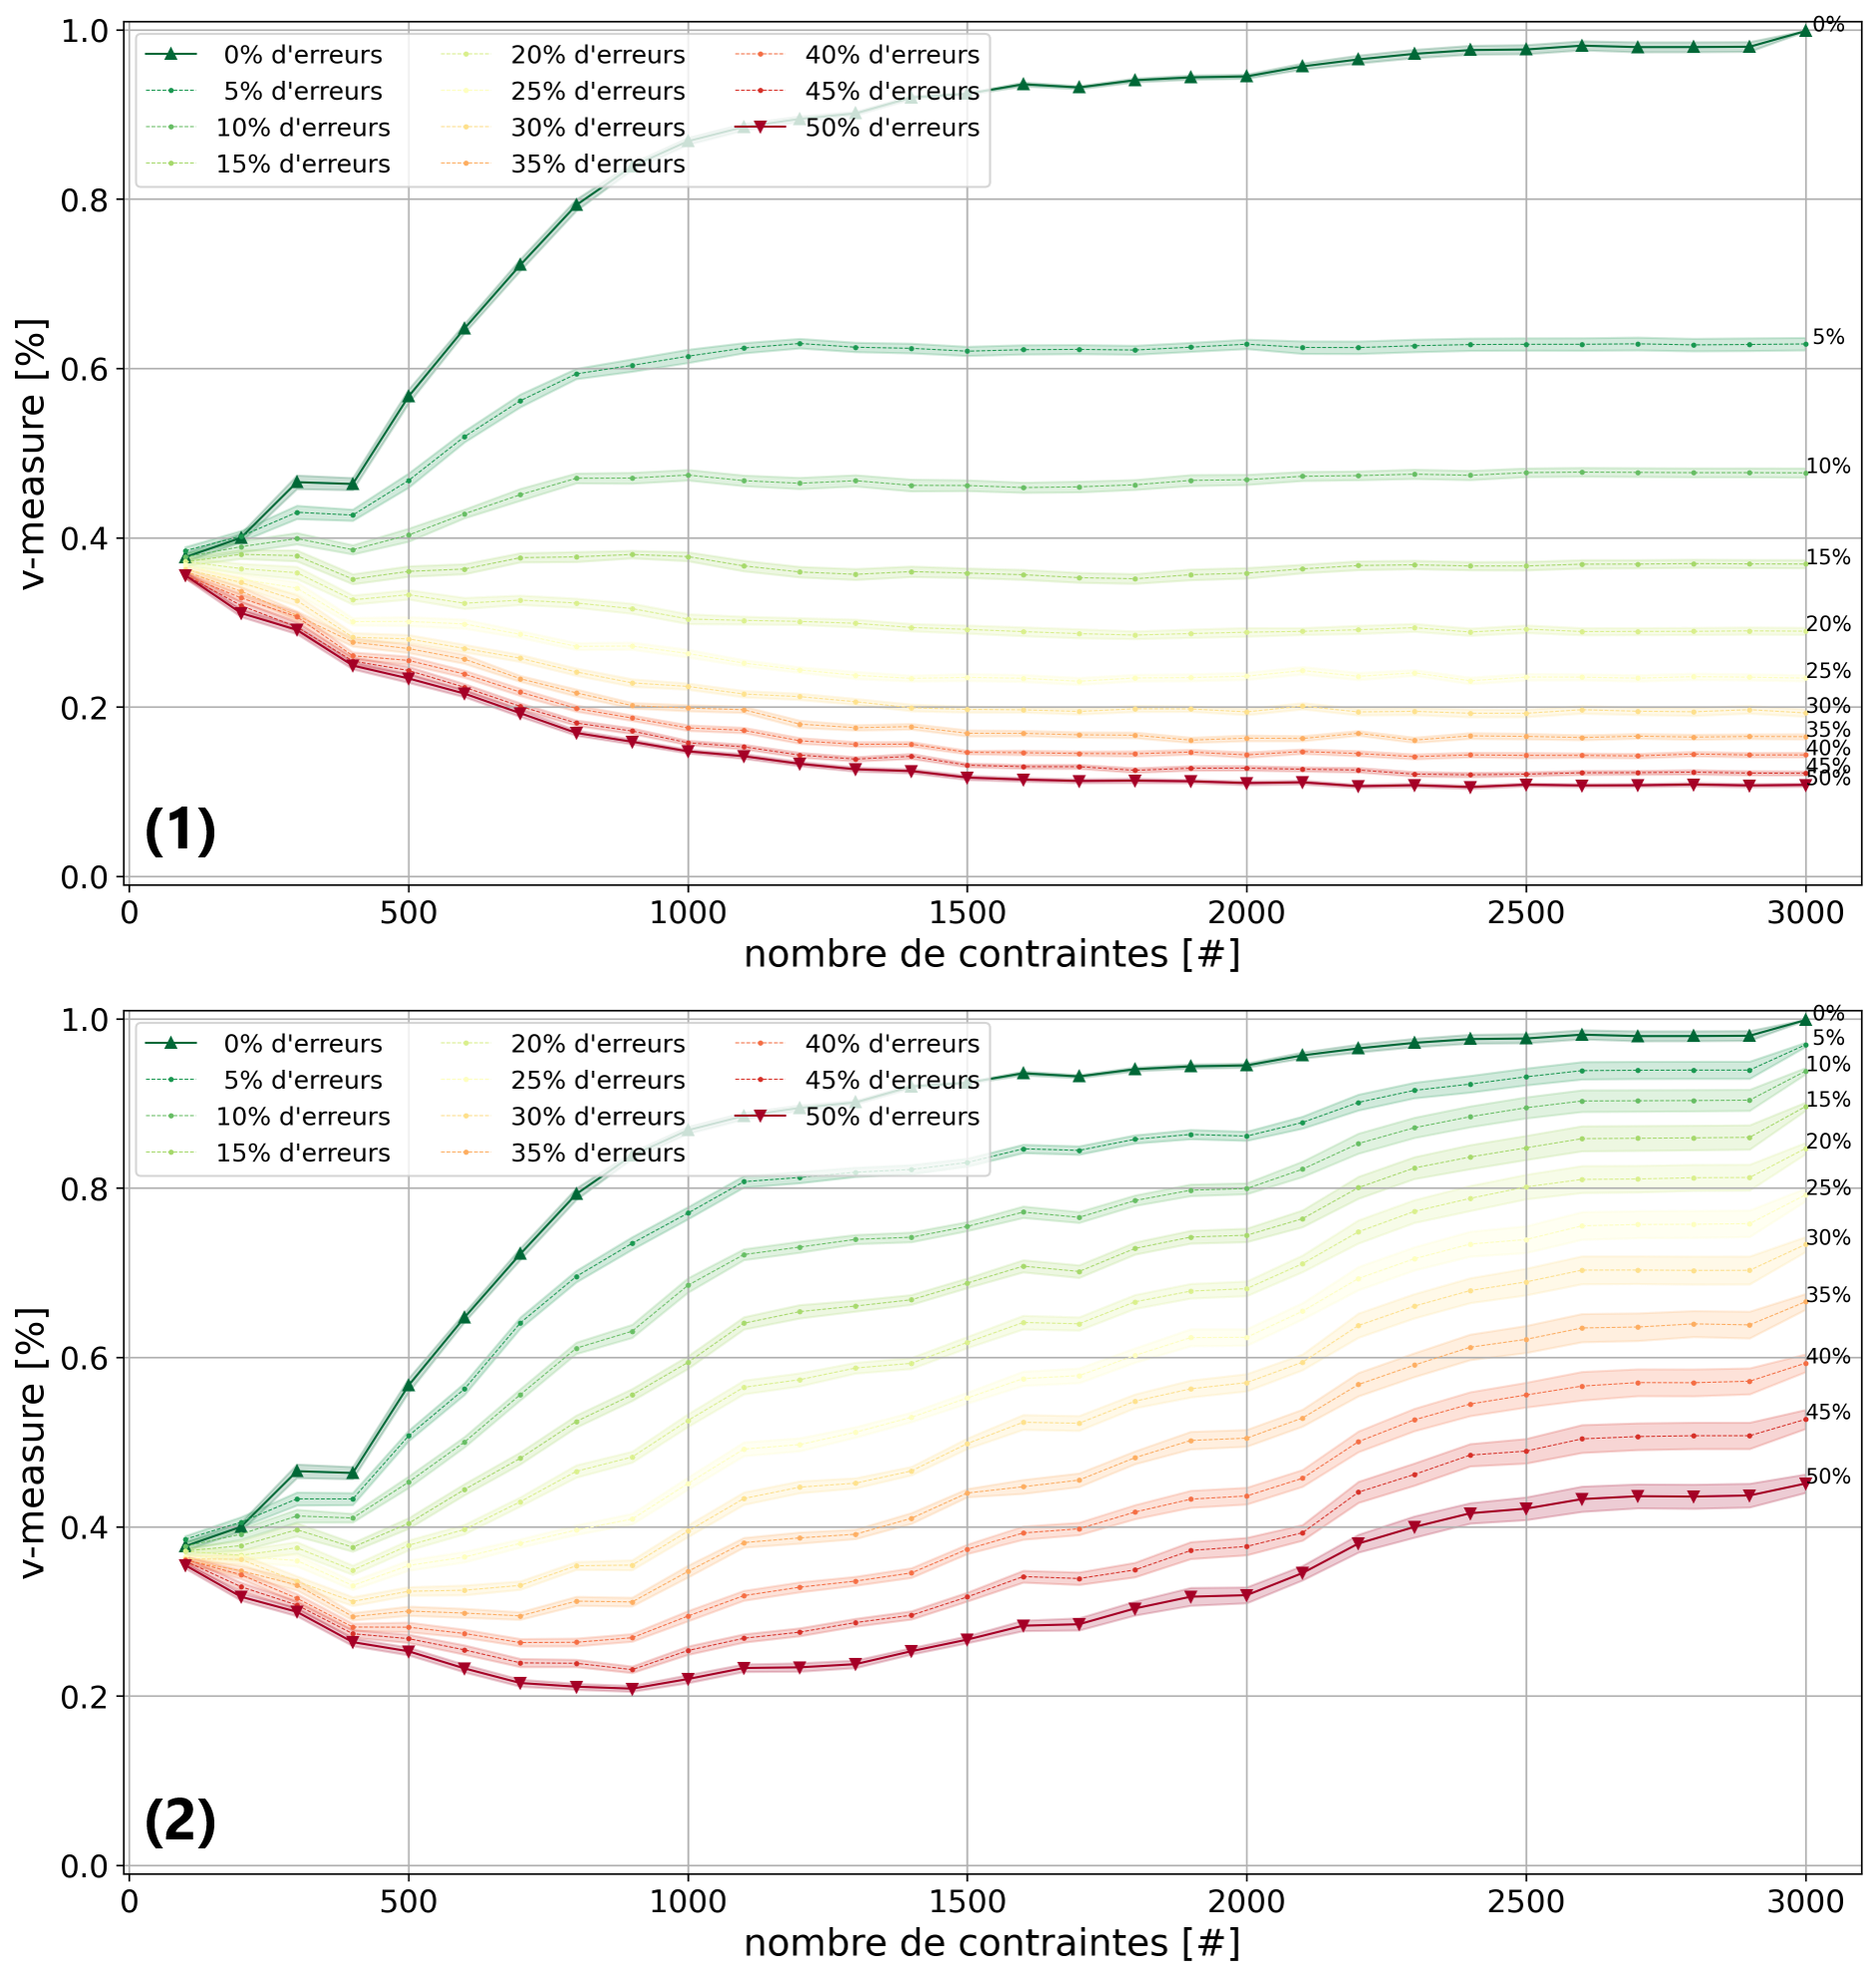
\includegraphics[width=0.95\textwidth]{figures/etude-erreur-simulation-impact-closest}
				\caption{
					Évolutions de la moyenne de la \texttt{v-measure} entre un résultat obtenu et la vérité terrain en fonction du nombre de contraintes annotées au cours des itérations du \textit{clustering} interactif.
					Les courbes en dégradé de couleur représentent les déclinaisons de cette évolution en intégrant un pourcentage d'annotations erronées (allant de $0$\% et $50$\%).
					\textbf{(1)} et \textbf{(2)} représente respectivement l'approche ignorant les conflits dans les contraintes et l'approche corrigeant les conflits détectés par le gestionnaire de contraintes.
					Toutes les courbes sont tronquées à $3~000$ contraintes.
				}
				\label{figure:4.6.1-ETUDE-ROBUSTESSE-INTERETS-CORRECTION-ERREURS}
			\end{figure}
			
			% Description de la figure.
			\todo[inline]{A REDIGER: description de la figure}

		%%% Discussion
		\subsubsection{Discussion}
		
			% Rappel de l'objectif : ...
			\todo[inline]{A REDIGER: rappel de l'objectif}
		
			% Remaques expérience utilisateur.
			\todo[inline]{A REDIGER: Super important de corriger !}
			\todo[inline]{A REDIGER: Besoin de mécanisme pour prédire et mettre de la redondance}
			
			% Conclusions et suggestion.
			\todo[inline]{A REDIGER: ouverture sur l'impact des incohérences}
	
	
	%%%
	%%% Subsection 4.6.2: Étude de l'impact des incohérences d'annotation sur les performances.
	%%%
	\subsection{Étude de l'impact des incohérences d'annotation sur les performances}
	\label{section:4.6.2-ETUDE-ROBUSTESSE-SIMULATION-IMPACT-ERREURS}
		
		% Objectif de l'expérience.
		\todo[inline]{A REDIGER: objectif de l'expérience}
	
		%%% Protocole expérimental.
		\subsubsection{Protocole expérimental}
			
			% Axiome.
			% Pseudo-code.
			% Détails de l'expérience.
			\todo[inline]{A REDIGER}
			
			% Référence scripts.
			\begin{leftBarInformation}
				Les scripts de l'expérience, réalisés avec des \textit{notebooks} Python (\cite{van-rossum-drake:2009:python-reference-manual}), sont disponibles dans un dossier dédié de~\cite{schild:2021:cognitivefactory-interactiveclusteringcomparativestudy}.
			\end{leftBarInformation}

		%%% Résultats
		\subsubsection{Résultats obtenus}
			\todo[inline]{A REDIGER}
		
			% Description statistiques.
			\todo[inline]{A REDIGER:}
			La \textsc{Table~\ref{table:4.6.2-ETUDE-ROBUSTESSE-SIMULATION-IMPACT-ERREURS}}
			
			\begin{table}[!htb]
				\begin{center}
				\begin{tabular}{|c|r|r|r|r|r|r|r|r|r|}
					% ENTETE DU TABLEAU
					% Erreur 0.00%
					% Erreur 0.05%
					% Erreur 0.10%
					% Erreur 0.15%
					% Erreur 0.20%
					% Erreur 0.25%
					% Erreur 0.30%
					% Erreur 0.35%
					% Erreur 0.40%
					% Erreur 0.45%
					% Erreur 0.50%
				\end{tabular}
				\end{center}
				\caption{
					Simulation ...
				}
				\label{table:4.6.2-ETUDE-ROBUSTESSE-SIMULATION-IMPACT-ERREURS}
			\end{table}

		%%% Discussion
		\subsubsection{Discussion}
		
			% Rappel de l'objectif : ...
			\todo[inline]{A REDIGER: rappel de l'objectif}
		
			% Remaques expérience utilisateur.
			\todo[inline]{A REDIGER: prédiction de retard}
			
			% Conclusions et suggestion.
			\todo[inline]{FIN}
			
			
	%%%
	%%% Subsection 4.6.3: Étude du score inter-annotateurs obtenu avec des opérateurs en situation réelle.
	%%%
	\subsection{Étude du score inter-annotateurs obtenu avec des opérateurs en situation réelle}
	\label{section:4.6.3-ETUDE-ROBUSTESSE-SCORE-INTER-ANNOTATEURS}
		
		% Objectif de l'expérience.
		Nous voulons étudier le score d'accord inter-annotateurs calculé lors d'une annotation de contraintes par plusieurs expert métiers en situation réelle.
		Pour cela, nous reprenons l'expérience de la \textsc{Section~\ref{section:4.3.1-ETUDE-COUTS-TEMPS-ANNOTATION}} visant à estimer le temps moyen d'annotation d'un lot de contraintes, et nous adaptons son protocole expérimental pour estimer l'accord inter-annotateurs.
		
	
		%%% Protocole expérimental.
		\subsubsection{Protocole expérimental}
			
			% Axiome.
			\begin{leftBarWarning}
				Dans cette étude, nous supposons que les annotateurs de l'expérience connaissent parfaitement le domaine traité dans le jeu de données, et qu'ils sont capables de caractériser sans ambiguïté la similitude entre deux données issues de cet ensemble.
				Afin de pourvoir faire cette hypothèse forte, et ainsi limiter les bruits dans l'analyse des résultats, le jeu de données devra traiter d'un sujet de culture générale (ne nécessitant donc pas de connaissance particulière) et des réviseurs supprimeront en amont et d'un commun accord les données trop spécifiques ou trop ambiguës.
			\end{leftBarWarning}
			
			% Pseudo-code.
			Pour résumer le protocole expérimental que nous décrivons ci-dessous, vous pouvez vous référer au pseudo-code décrit dans \textsc{Algorithme~\ref{algorithm:4.6.3-ETUDE-ROBUSTESSE-SCORE-INTER-ANNOTATEURS-PROTOCOLE}}.

			\begin{algorithm}
				\KwData{jeu de données annoté (vérité terrain)}
				\KwIn{plusieurs réviseurs, plusieurs annotateurs}
				%
				\textbf{initialisation}: définir et revoir le jeu de données entre réviseurs \;
				\textbf{échantillonnage}: sélectionner une base de contraintes équilibrée \;
				\ForEach{annotateur}{
					 \While{la base de contraintes n'a pas été entièrement annotée}{
						\textbf{annotation}: annoter une partie des contraintes \;
						\textbf{revue}: revue des contraintes en conflits d'annotation \;
					}
				}
				%
				\KwResult{modélisation du score inter-annotateurs sur le lot de contraintes}
				%
				\caption{\textit{
					Description en pseudo-code du protocole expérimental de l'étude du score inter-annotateurs d'annotation d'un lot de contraintes par plusieurs experts métiers en situation réelle.
				}}
				\label{algorithm:4.3.3-ETUDE-COUTS-TEMPS-ANNOTATION-PROTOCOLE}
			\end{algorithm}
			
			% Détails de l'expérience : préparation du jeu de données.
			Nous allons procéder en plusieurs étapes.
			D'abord, il faut choisir un jeu de données approprié : pour valider notre hypothèse forte sur les compétences de nos annotateurs, nous cherchons un jeu de données traitant d'un sujet de culture général.
			Pour cette expérience, nous avons donc choisi \texttt{MLSUM} : une collecte d'articles de journaux, classés par catégorie de publication et décrits par leur titre et leur résumé.
			Nous nous intéressons ici à la tâche de classification d'un titre d'article en fonction de sa catégorie de publication.
			Comme certains titres peuvent porter à confusion (un titre d'article n'étant pas toujours explicite sur son contenu), deux réviseurs sont chargés de choisir les données les plus explicites sur un échantillon d'un millier de données représentatives des catégories les plus communes.
			L'échantillon résultant, noté \texttt{MLSUM FR Train Subset (v1.0.0-schild)}, est composé de $744$ titres d'articles rédigés en français et répartis en $14$ classes (\textit{économie}, \textit{sport}, ...).
			Pour plus de détails, consultez l'annexe~\ref{annex:C.2-DATASET-MLSUM-SUBSET-SCHILD}.
		
			% Détails de l'expérience : sélection des contraintes à annoter.
			A partir de ces données, nous sélectionnons un lot de $400$ contraintes à annoter.
			Pour faciliter l'analyse, l'échantillonnage sera un aléatoire équilibré d'après la vérité terrain en $200$ \texttt{MUST-LINK} et en $200$ \texttt{CANNOT-LINK}.
			
			% Détails de l'expérience : annotations et consignes.
			Ensuite, un groupe de $3$ annotateurs vont annoter la sélection de $400$ contraintes en plusieurs sessions.
			Les directives données aux opérateurs sont les suivantes:
			\begin{itemize}
				\item \textbf{Contexte de l'opérateur} :
				\textguillemets{\textit{Vous êtes des \textbf{experts de la presse et de l’actualité} ; Vous voulez classer des articles dans des catégories en fonction de leur titre ; Vous ne savez pas précisément quelles catégories vous allez utiliser pour classer vos articles ; Mais vous savez \textbf{caractériser la similitude} de deux articles}} ;
				\item \textbf{Contexte sur le jeu de données} :
				\textguillemets{\textit{Le thème sont les catégories d’articles de presse ; La vérité terrain contient entre $10$ et $20$ catégories parmi les plus communes de la presse ; La vérité terrain contient entre $30$ et $100$ articles par catégorie ; Vous \textbf{pouvez regarder le jeu de données non annoté} autant que vous le voulez (disponible dans l'onglet \texttt{TEXTS} de l'application)}} ;
				\item \textbf{Consignes d'annotations} :
				\textguillemets{\textit{Faites des séries de \textbf{15 minutes minimum} pour avoir de la régularité ; Si possible, \textbf{isolez-vous} pour ne pas être dérangé et ne pas fausser les résultats ; Pour chaque série, \textbf{notez le temps et le nombre de contraintes annotés} ; Si vous ne savez pas quoi annoter (trop ambigu, vocabulaire inconnu, ...), \textbf{passez au suivant sans annoter} (vous êtes sensés être des experts de la presse !)}}.
			\end{itemize}
			%
			Pour réaliser l'annotation, les opérateurs auront accès à l'application web développée au cours de ce doctorat.
			Des captures d'écran sont disponibles en \textsc{Figure~\ref{figure:4.3.1-ETUDE-COUTS-TEMPS-ANNOTATION-APPLICATION-ANNOTATION}} et \textsc{Figure~\ref{figure:4.3.1-ETUDE-COUTS-TEMPS-ANNOTATION-APPLICATION-LISTE-CONTRAINTES}}.
			Une description plus détaillée de l'application et de ses fonctionnalités est disponible en \textsc{Section~\ref{section:3.3-DESCRIPTION-IMPLEMENTATION}}\todo{description à faire}.
			
			% Détails de l'expérience.
			\todo[inline]{A REDIGER / A COMPLETER}
			
			% Référence scripts.
			\begin{leftBarInformation}
				Les scripts de l'expérience, réalisés avec des \textit{notebooks} Python (\cite{van-rossum-drake:2009:python-reference-manual}), sont disponibles dans un dossier dédié de~\cite{schild:2021:cognitivefactory-interactiveclusteringcomparativestudy}.
			\end{leftBarInformation}
			
		%%% Résultats
		\subsubsection{Résultats obtenus}
		
			% Description statistiques.
			La \textsc{Table~\ref{table:4.6.3-ETUDE-ROBUSTESSE-SCORE-INTER-ANNOTATEURS}} expose les scores inter-annotateurs sur les $3$ opérateurs et le réviseur de cette expérience, ainsi que l'accord avec la vérité terrain.
			Le score d'accord moyen avec la vérité terrain est de $0.86$ (écart-type: $0.01$) ; ce score est de $0.81$ (écart-type: $0.05$) pour les contraintes de types \texttt{MUST-LINK} et est de $0.92$ (écart-type: $0.03$) pour les contraintes de types \texttt{CANNOT-LINK}.
			Le score inter-annotateurs moyen (sans le réviseur) est de $0.84$ (écart-type: $0.03$).
			
			\begin{table}[!htb]
				\begin{center}
				\begin{tabular}{|c|r|r|r|r|}
				
					\hline
					% ENTETE DU TABLEAU
					
						& \multicolumn{1}{c|}{\shortstack[c]{
							1 (Relecteur)
						}}
						& \multicolumn{1}{c|}{\shortstack[c]{
							7 (Annotateur)
						}}
						& \multicolumn{1}{c|}{\shortstack[c]{
							9 (Annotateur)
						}}
						& \multicolumn{1}{c|}{\shortstack[c]{
							12 (Annotateur)
						}}
						\tabularnewline
						\hline

					% Vérité terrain
					\multicolumn{1}{|c|}{\shortstack[c]{
						Vérité terrain
					}}
						& $0.95$
						& $0.86$
						& $0.84$
						& $0.87$
						\tabularnewline
						\hline

					% Vérité terrain
					\multicolumn{1}{|c|}{\shortstack[c]{
						1 (Relecteur)
					}}
						&
						& $0.91$
						& $0.86$
						& $0.89$
						\tabularnewline
						\hline

					% Vérité terrain
					\multicolumn{1}{|c|}{\shortstack[c]{
						7 (Annotateur)
					}}
						&
						&
						& $0.86$
						& $0.85$
						\tabularnewline
						\hline

					% Vérité terrain
					\multicolumn{1}{|c|}{\shortstack[c]{
						9 (Annotateur)
					}}
						&
						&
						&
						& $0.80$
						\tabularnewline
						\hline
					
				\end{tabular}
				\end{center}
				\caption{
					Score d'accord inter-annotateurs obtenu avec $1$ réviseur et $3$ annotateurs sur un lot commun de $400$ contraintes ($200$ \texttt{MUST-LINK}, $200$ \texttt{CANNOT-LINK}).
				}
				\label{table:4.6.3-ETUDE-ROBUSTESSE-SCORE-INTER-ANNOTATEURS}
			\end{table}
			
			% Note.
			\begin{leftBarInformation}
				Dans une autre expérience, où $14$ opérateurs devaient annoter une base de $1~000$ contraintes aléatoires, nous obtenons un accord moyen avec la vérité terrain de $0.93$ (écart-type: $0.02$) et un score inter-annotateurs moyen de $0.91$ (écart-type: $0.03$).
				Toutefois, nous ne mettons pas en avant ces résultats car le lot de contraintes à annoté est déséquilibré à cause de l'utilisation de l'échantillonnage aléatoire ($932$ \texttt{CANNOT-LINK}, $68$ \texttt{MUST-LINK}).
			\end{leftBarInformation}
	
		%%% Discussion
		\subsubsection{Discussion}
		
			% Rappel de l'objectif : ...
			\todo[inline]{A REDIGER: rappel de l'objectif}
		
			% Avantage 1 : peu d'erreurs
			\todo[inline]{A REDIGER: Peu d'erreurs (environ 16\% d'erreurs sans concertations)}
			
			% Remarque 1 : MUST-LINK < CANNOT-LINK
			\todo[inline]{A REDIGER: CANNOT-LINK légèrement plus facile que les MUST-LINK}
			
			% Conclusions et suggestion.
			\todo[inline]{A REDIGER: ouverture sur l'impact des non-corrections}
			
	%%%
	%%% Subsection 4.6.3: Bilan concernant la robustesse du \textit{clustering} interactif
	%%%
	\subsection{Bilan concernant la robustesse du \textit{clustering} interactif}
	\label{section:4.6.3-ETUDE-ROBUSTESSE-MISE-EN-COMMUN}
	
		\todo[inline]{A REDIGER}
	
		% Conclusion.
		\begin{leftBarSummary}
			Au cours de cette étude de pertinence, nous avons pu voir que :
			\begin{itemize}
				\item[\itemok] ...
				\item[\itemok] ...
				\item[\itemok] ...
			\end{itemize}
		\end{leftBarSummary}